\documentclass{article}

\usepackage{times}
\usepackage{geometry}
\geometry{a4paper,left=0.6cm,right=0.7cm,top=1cm,bottom=1cm,columnsep=0.8cm}

\usepackage{fontawesome}
\usepackage[hidelinks]{hyperref}
\usepackage{multicol,paracol,tikz,hyphsubst,moresize,hyphenat,adjustbox,tabularx,xcolor,enumitem}
\newcolumntype{Y}{>{\RaggedRight\arraybackslash}X}
\setlist[itemize]{itemsep=1pt,leftmargin=*,topsep=-10pt}

\definecolor{maincolor}{HTML}{ffffff}
\definecolor{seccolor}{HTML}{0b1f3b}
\definecolor{gray}{HTML}{8c94a9}
\definecolor{sidetext}{HTML}{59cee5}
\definecolor{Green}{HTML}{2caf00}
\definecolor{lightgray}{HTML}{D3D3D3}

% --- bande latérale bleue
\usepackage{eso-pic}
\AddToShipoutPictureBG{%
  \begin{tikzpicture}[remember picture,overlay]
    \fill[seccolor] (0.7\paperwidth,0) rectangle (\paperwidth,\paperheight);
    \fill[maincolor] (0,0) rectangle (0.7\paperwidth,\paperheight);
  \end{tikzpicture}%
}

\setlength{\parindent}{0pt}
\newcommand{\cvsection}[1]{%
  \par\bigskip                % espace avant le titre
  {\bfseries\Large #1}\par
  \noindent\rule{\linewidth}{0.8pt}\par
  \medskip                    % espace après la ligne
}

\newcommand*{\ClipSep}{0.4cm}

% ------------------------------------------------------------------
\begin{document}\pagestyle{empty}
\columnratio{0.7}\begin{paracol}{2}

% --------- colonne gauche -----------------------------------------
\begin{minipage}{0.7\linewidth}
{\LARGE\textbf{Pape Saliou Fall}}

\bigskip
{\large\textbf{Ingénieur Data Scientist \& Développeur IA}}
\end{minipage}\hfill
\begin{minipage}{0.18\linewidth}
\begin{tikzpicture}
\node[inner sep=0pt]{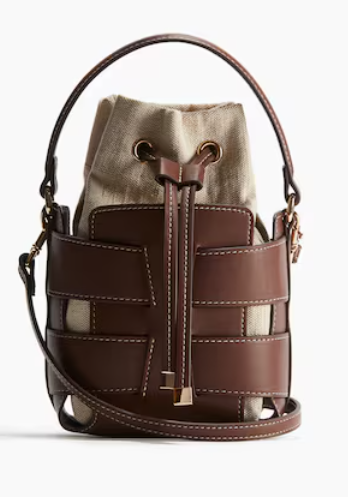
\includegraphics[width=\linewidth]{d0aeaf04bbf64a9ca35058c782c94388.png}};
\draw[white,rounded corners=\ClipSep,line width=\ClipSep]
      (current bounding box.north west) --
      (current bounding box.north east) --
      (current bounding box.south east) --
      (current bounding box.south west) -- cycle;
\end{tikzpicture}
\end{minipage}

\cvsection{Profil}
Data Scientist et développeur IA passionné, je conçois des solutions qui transforment des données complexes en leviers décisionnels. Ma double compétence en science des données et en développement full-stack me permet de bâtir des plateformes intelligentes de bout en bout. Curieux, autonome et proactif, j’aime relever des défis techniques et collaborer avec des équipes pluridisciplinaires. Mon ambition : contribuer à des projets innovants à fort impact.

\cvsection{EXPÉRIENCE}

\colorbox{maincolor}{%
  \begin{minipage}{\linewidth}
    \textbf{Data Scientist \& Développeur IA} \\ Prepaya \\ janv. 2024 – présent
    \begin{itemize}
      \item Conçu et déployé une plateforme IA full-stack (Python/JavaScript) dédiée à l’analyse de séries temporelles et à la prédiction en temps réel. \item Implémenté des modèles de machine et deep learning avec Scikit-learn, TensorFlow et Keras pour améliorer la précision des prévisions. \item Intégré l’API OpenAI, PostgreSQL et le cloud Heroku afin d’automatiser le pipeline de données de bout en bout.
    \end{itemize}
  \end{minipage}}

\vspace{3mm}


\colorbox{maincolor}{%
  \begin{minipage}{\linewidth}
    \textbf{Apprenti Risk Analyst \& Data Scientist} \\ AXA XL (Groupe AXA) \\ déc. 2022 – déc. 2023
    \begin{itemize}
      \item Automatisé la collecte des données financières, réduisant les manipulations manuelles et fiabilisant le reporting. \item Créé des tableaux de bord Power BI pour suivre la facturation et soutenir les équipes finance, gestion et direction. \item Développé des applications prédictives évaluant le risque de sinistre client via modèles statistiques et machine learning.
    \end{itemize}
  \end{minipage}}

\vspace{3mm}


\colorbox{maincolor}{%
  \begin{minipage}{\linewidth}
    \textbf{Apprenti Data Scientist} \\ Prepaya \\ sept. 2021 – août 2022
    \begin{itemize}
      \item Déployé des modèles NLP (T5, BERT) pour générer automatiquement des formulaires clients. \item Réalisé une analyse de sentiments des retours clients afin d’identifier les thèmes de satisfaction et d’amélioration. \item Automatisé la collecte et le pré-traitement de données textuelles avec Python (BeautifulSoup, Selenium).
    \end{itemize}
  \end{minipage}}

\cvsection{FORMATION}

    \begin{tabularx}{\linewidth}{@{}c X@{}}
    \textcolor{sidetext}{\faGraduationCap} &
    \textbf{Master 2 Data Science} \\
    & Sorbonne Université, Paris \\
    & \begin{itemize}[leftmargin=*]
  \item Analyse de données avancée, séries temporelles et calcul parallèle. \item Modélisation statistique, machine learning et deep learning. \item Conception de bases de données et déploiement d’applications d’IA.
\end{itemize} \\
    & \textit{sept. 2021 – mars 2022}
    \end{tabularx}
    

% --------- colonne droite (bleue) ---------------------------------
\switchcolumn\color{white}\hspace*{0.4cm}\begin{minipage}{0.88\linewidth}

\cvsection{CONTACT}
\begin{tabular}{@{}c l}
  \faPhone & \href{tel:0753481453}{0753481453} \\[2pt]
  \faEnvelope & \href{mailto:papesalioufall2@gmail.com}{papesalioufall2@gmail.com} \\[2pt]
  \faMapMarker & 95300 Pontoise\\ \\[2pt]
  \faLinkedin & \href{pape-saliou-fall-43154a211}{pape-saliou-fall-43154a211}
\end{tabular}

\cvsection{COMPÉTENCES}

\begin{itemize}[leftmargin=*]
\item Python
\item SQL
\item PowerBI
\item Git
\item TensorFlow
\item Scikit
\item Flask\end{itemize}
\par\bigskip 

\cvsection{LANGUES}
\begin{itemize}[leftmargin=*]
\item Français - \textcolor{gray}{Maternel}
\item Anglais - \textcolor{gray}{B2}\end{itemize}
\par\bigskip 
\cvsection{INTÉRÊTS}
\begin{itemize}[leftmargin=*]
\item Football
\item Natation
\item Lecture
\end{itemize}

\end{minipage}
\end{paracol}
\end{document}
